\chapter{Introduction}
	\label{chapter:Introduction}
	\section{Introduction}
	
"`Soundgates – Interactive Music Synthesis on FPGAs"' is a project initiated by the Computer Engineering Group of the University of Paderborn, aiming to synthesise music on modern FPGAs. 
Furthermore, one or more users should use this interactive system, by means of manipulating the synthesised music with advanced sensors such as the acceleration sensor in modern smartphones.
	

	
	
	\section{About this document}
	This document is the project plan of the project group ``Soundgates'' at the University of Paderborn. 
	

	Not only should this document serve as a basis for the later evaluation and grading by our professor, but also as a reference for our group during the main working phase.
	This working phase runs from ??.2013 to ??.2014
	\section{Definitions}
	 The following table displays some definitions, that will be used throughout this document.\\
	
	 \begin{tabular}[h]{|c|p{9.75cm}|}
	  \hline
	  Term & Definition \\
	  \hline
	  \hline
	  Composite Component & Definition \\\hline
	  Component & A basic building block to generate music ??Haben wir uns hier auf Block als Bezeichnung geeinight? Component eher im Sinne von Softwarekomponente\\\hline
	  Editor & The Editor is used to create a patch out of components to generate synthesizable code which can be put on a FPGA \\\hline
	  FPGA & Field Programmable Gate Array \\\hline
	  Patch & The entire system which consists of Components and Composite Components. A set of single Components can build a new Component \\\hline
	  Port & The interface from one Component to another one \\\hline
	  Simulation & The developed patch is played through the PC speakers \\\hline
	 \end{tabular}
	 

	\section{Generative music}
	

	\subsection{Introduction}

	As pointed out in \cite{Chandra2012}, there are many cultures where musicical experience is defined by people performing and people perceiving music. 
	The only way to slightly exert influence on the performer's music is by cheering, shouting, etc. on a concert. 
	The gap between performer and perceiver reaches its peak in the context of recorded music like CDs or MP3 files, where is no chance of manipulate the music. 
	Actually, there is a rising trend for interacticing with music on your own or with a familiar social partner, like in the video game "`Guitar Hero"' \cite{Chandra2012, Planck2009}. 
	Even without any musical knowledges or talent, it is more and more possible to interact, manipulate or even create music.
	Generative music combines the opportunities of making music without having knowledges of how to play an instrument and explicitly exert influence on music you hear.
	An early an popular example for generative music was Mozart's musical dice game. Given a set of small sections of music, it was randomly chosen which part was played next.



	\subsection{Approaches} 

	Genarative music (or algorithmic music) can be devided into the following subcategories \cite{Wooller2005}.

	\subsubsection{Linguistic/Structural}

	Already existing songs are scanned in the first place and afterwards recomposed randomly. Therefore, a grammer is created where the production rules are made of sequent pairs of notes. The generation of the new song is achieved by executing this production rules randomly.

	\subsubsection{Creative/Procedural}

	There are different processes/procedures which play predefined music. This processes have an arbitrary order and starting time. A popular is Mozart's musical dice game. 

	\subsubsection{Biological Emergent}

	Music is generated by biological phenomenons, i.\,e. by differing parameters within an ecology, for example wind-chimes.

	\subsubsection{Interactive/Behavioural}

	The interactive/behavioural generative music approach results from processes without discernable musical inputs. It is a question of synthesized music and recorded and filtered samples at the most. The music generation is fully controlled by user input and interaction.
	
	This is the initial point on what this project is based: synthesizing music along with a highly interactive interface to exert influence on the music.

	\section{Possible User Interactions}
	In order to make the system interactive there need to be one or more interfaces, over which the user can take influence on the music. This could happen via midi keyboard or other electronic instruments. But with the purpose of providing an easy, playful access to music generation without knowledges of an instruments, we are focussing on advanced sensors. Sensors like Microsoft's Kinect systems can easily track e.\,g. the user's hand. An intuitive way of changing system's parameters is to measure and transmit the height of the hand. Other possible sensors can be found in nearly every modern smartphone, e.\,g. the acceleration sensors.
	
			
				
	\section{Introduction to sound synthsis}
		The easiest way to generate sound on a digital system, e.\,g. on a computer, is basicly originated from analog synthesizers. The main idea to generate waveforms, such as a basic sine wave. The digital stored values of the wave are then fed into an Digital-Analaog-Converter (DAC), which converts the values to an analog signal. These signals are now able to be played on a speaker. Figure \ref{fig:sound_generation} depicts this easy example. Advanced ways of generating sounds would be with additional waveforms, filters and arithmetic functions.
	
	  	\begin{figure}[!h]
		\centering
			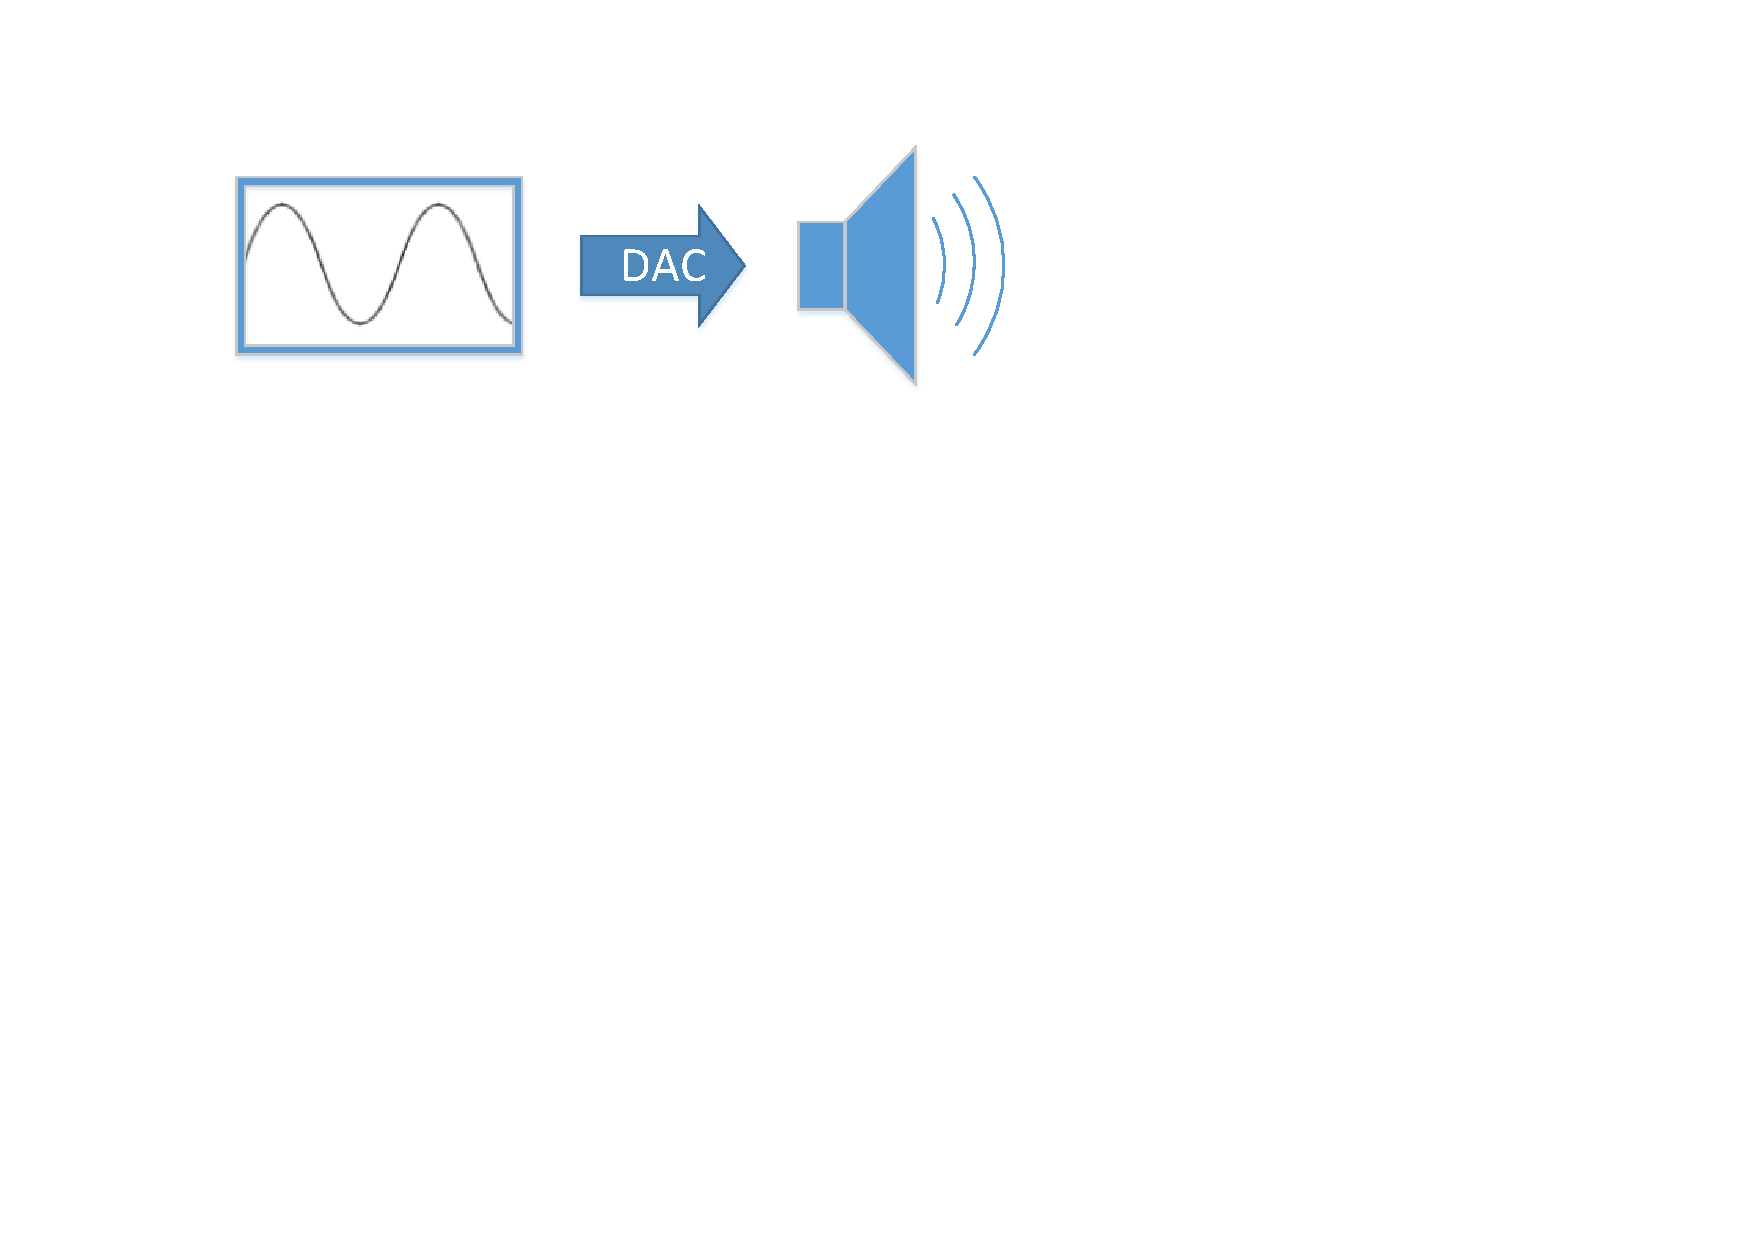
\includegraphics[width=0.90\textwidth]{images/sound_generation.pdf}
		\caption{Easiest way to generate sound on a digital system}
		\label{fig:sound_generation}
	\end{figure}
		
		
		
		
		%- Artifical generation of sound
	  %- Generation of basic waveforms
	    %- More complex and rich patterns by methods like additive/subtractive/... synth 
	  %- Further addition of filters etc
	  %
	  %- Originated from analog synthesizers, nowadays mostly digital. Software for general purpose PCs exist
	  %
	  %- Building patches: job of a sound designer, rather than a musician
			
			
			
			%\section{Project outline}  -- das steht in goals oder?
	  %- Creating an editor for synthesizers. 
	  %- Components of the synthesizer implemented in hardware (and software for simulation purpose)
	  %- Implementation of generative music concepts
	  %------- Warum wollen wir das eigentlich tun? Was ist die Motivation dahinter (zumal es das aus Oslo ja aschon in Software gibt)
		
	\section{Employed systems}
	  \subsection{Xilinx Platform Studio}
	    The overall hardware system is implemented in VHDL, using the Xilinx Platform Studio (XPS), which offers the MicroBlaze Softcore Processor.
	  \subsection{ReconOS}
		ReconOS is an Operating System which can be run on a softcore CPU on a FPGA. Through it's support for the Linux kernel it is possible to write applications which consist of Hard- and Software threads. Therefore the software threads can be used to communicate via sockets with sensors and hand over these values to the hardware threads, which are responsible for generating sounds.
	  \subsection{Eclipse/GMF}
		We avoid building a new graphical editor from ground up since this is an error prone process. Instead we rely on the Model Driven Software Development process for graphical editors which is provided by the GMF framework. Therefore we can generate an editor by specifing the Meta-Model. The graphical surface with our components are connections are the result. Additionally it is neccessary to provide functions for every component, so it will be possible to simulate the generated output.
	  
		\section{Document Structure}
		First of all the goals we want to achieve are described in Chapter \ref{chapter:Goals}. Chapter \ref{chapter:RelatedWork} covers systems similar to what we are going to create, escpecially the software 
		called MAX.	Chapters \ref{chapter:Organization} and \ref{chapter:Workplan} describe how the group will organize itself and the groups' milestones.
      